\section{Cronograma}
\label{cronograma}
%Distribución de actividades a lo largo del tiempo de ejecución del
%proyecto. Asociar a cada actividad el o los objetivos (numerados)
%relacionados con estos. 

El cronograma est\'a estructurado a partir de las tareas y
responsables especificadas en la Seccion \ref{metodologia}.  

El diagrama de Gantt se muestra en la Figura \ref{gantt}.

\begin{figure}
\begin{center}
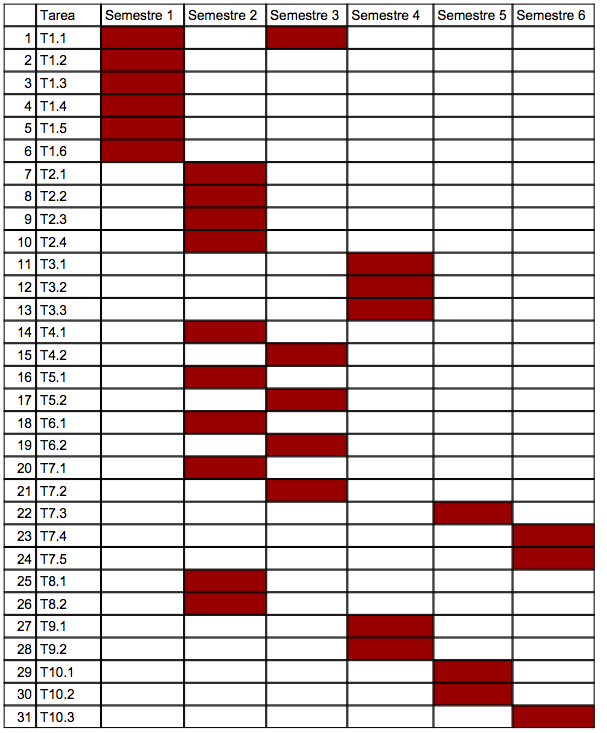
\includegraphics[width=0.80\textwidth]{gantt_chart.png}
\end{center}
\caption{Diagrama de Gantt que resume la repartici\'on de tareas del
  cronograma (Secci\'on \ref{cronograma}). 
\label{gantt}}
\end{figure}

\begin{itemize}
\item[\bf SEM-1]
\begin{itemize}
\item[T1.1] \tecn Compra, instalaci\'on y mantenimiento de 3TB espacio de disco
  con backup para almacenar los datos originales de las simulaciones.
\item[T1.2] \tecn Compra, instalaci\'on y mantenimiento de un blade de
  procesamiento con 24 procesadores con 512GB para poder analizar y
  postprocesar las simulaciones.
\item[T1.4] \gradA\prof Instalaci\'on del software abierto {\texttt N-GenIC}\footnote{\url{http://www.mpa-garching.mpg.de/gadget/}} para la generaci\'on de condiciones iniciales.
\item[T1.3] \gradA\prof Instalaci\'on del software abierto {\texttt
  Gadget2}\footnote{\url{http://www.mpa-garching.mpg.de/gadget/}} para hacer simulaciones de N-cuerpos cosmol\'ogicas.
\item[T1.5] \gradA\prof Instalaci\'on del sofware abierto {\texttt
  Rockstar}\footnote{\url{https://bitbucket.org/gfcstanford/rockstar}} para la detecci\'on de halos de materia oscura.
\item[T1.6] \gradA\gradB\prof Organizaci\'on de una escuela internacional en
  cosmolog\'ia computational (duraci\'on de un mes) para formar
  recurso humano con capacidad de utilizar hardware y software para
  hacer y analizar simulaciones de formaci\'on de estructura a gran
  escala. Dr. Stefan Gottloeber ser\'a uno de los profesores.
\end{itemize}


\item[{\bf SEM 2}]
\begin{itemize}

\item[T4.1] \gradA\prof Escribir software para la generaci\'on de cat\'alogos
  ficticios de galaxias aleatorios (i.e. sin ning\'un tipo de
  clustering). 
\item[T5.1] \prof Escribir software que simule la secuencia de observaci\'on
  de DESI sobre un cat\'alog de galaxias generado aleatoriamente. \bob.
\item[T6.1] \prof Escribir software que simule la asignaci\'on de fibras
  \'opticas sobre un cat\'alog de galaxias generadas aleatoriamente.  \bob.
\item[T7.1] \prof Integrar en la base de c\'odigo de DESI el software para
  preparar cat\'alogos ficticios de galaxias aleatorios. \bob. Viaje a Berkeley por dos semanas. 

\item[T2.1] \gradA Generar las condiciones iniciales para 5 vol\'umenes
  cosmol\'ogicos. 
\item[T2.2] \gradA Correr las simulaciones para 5 vol\'umenes LCDM.
\item[T2.3] \gradA Controlar la calidad de los 5 vol\'umenes LCDM.  
Esto se har\'a con la asesor\'ia de Dr. Stefan Gottloeber.
\item[T2.4] \gradA Identificar los halos de materia oscura en los 5
  vol\'umenes LCDM.
\item[T8.1] \gradB Medir la intensidad del efecto AP sobre cat\'alogos
  ficticios de galaxias creados a partir de simulaciones de N-cuerpos.\park
\item[T8.2] \prof Medir la intensidad del efecto AP sobre observaciones
  reales de galaxias. \park. Viaje a Seul por dos semanas.
\end{itemize}


\item[\bf SEM-3]
\begin{itemize}
\item[T1.1] \tecn Compra, instalaci\'on y mantenimiento de 3TB espacio de disco
  con backup para almacenar los datos originales de las simulaciones.
\item[T4.2] \gradA\prof Adaptar el c\'odigo {\texttt
  make\_survey}\footnote{\url{https://github.com/mockFactory/make_survey}}
  para generar  cat\'alogos fictios de galaxias a partir de
  cat\'alogos de halos materia oscura. 
\item[T5.2] \prof Escribir software que simule la secuencia de observaci\'on
  de DESI sobre un cat\'alogo de galaxias generado a partir de una
  simulaci\'on de N-cuerpos. \bob.
\item[T6.2] \prof Escribir software que simule la asignaci\'on de fibras
  \'opticas sobre un cat\'alog de galaxias generado a partir de una
  simulaci\'on de N-cuerpos. \bob.
\item[T7.2] \gradA\prof Integrar en la base de c\'odigo de DESI el software para
  preparar cat\'alogos ficticios de galaxias a partir de simulaciones
  de N-cuerpos. \bob. Viaje a Berkeley por 2 semanas.
\end{itemize}

\item[\bf SEM-4]
\begin{itemize}
\item[T3.1] \gradA Correr 5 simulaciones $w$CDM para las mismas condiciones 
  iniciales pero diferentes valores de $w$. 
\item[T3.2] \gradA Controlar la calidad de los 5 vol\'umenes $w$CDM. Esto se
  har\'a con la asesor\'ia de Dr. Stefan Gottloeber. 
\item[T3.3] \gradA Identificar los halos de materia oscura en los 5 vol\'umenes $w$CDM. 
\item[T9.1] \gradB\prof Cuantificar el n\'umero de pares de c\'umulos de galaxias  con velocidades extremas en simulaciones de N-cuerpos en
  cosmolog\'ias LCDM. 
\item[T9.2] \gradB Cuantificar el n\'umero de pares de c\'umulos de galaxias con velocidades extremas en simulaciones de N-cuerpos en
  cosmolog\'ias $\omega$CDM. Viaje a Seul por 2 semanas.
\end{itemize}


\item[\bf SEM-5]
\begin{itemize}
\item[T7.3] \prof Integrar en la base de c\'odigo de DESI el software para
  definir las secuencias de observaci\'on del experimento. \bob.
\item[T10.1] \gradB
  Cuantificar el efecto de RSD sobre cat\'alogos ficticios de
  galaxias creados a partir de simulaciones de N-cuerpos en
  cosmolog\'ias LCDM. 
\item[T10.2] \gradB Cuantificar el efecto de RSD sobre cat\'alogos ficticios de
  galaxias creados a partir de simulaciones de N-cuerpos en
  cosmolog\'ias $\omega$CDM. 
\end{itemize}

\item[\bf SEM-6]
\begin{itemize}
\item[T7.4] \prof Integrar el c\'odigo completo de simulaci\'on end-to-end
  de DESI. \bob. 
\item[T7.5] \prof Producir simulaciones completas de simulaci\'on end-to-end
  de DESI. Desde las observaciones hasta la estimaci\'on de redshifts
  de galaxias observadas. \bob. Visita a Berkeley por 2 semanas.
\item[T10.3] \gradB Cuantificar el efecto de RSD sobre los cat\'alogos de
  posiciones y redshift creados a partir de la herramienta de
  simulaci\'on end-to-end de DESI.\bob Visita a Berkeley por 2 semanas.
\end{itemize}

\end{itemize}
